\documentclass{beamer}

\usepackage{beamerthemesplit}
\usepackage{graphicx}
\usepackage{subfigure}
\usepackage{amsmath,amssymb}
\usepackage{multimedia}
\usepackage{times}
\usepackage{ulem}

\usepackage[latin1]{inputenc}
\usepackage[T1]{fontenc}
\usepackage{listings}
\usepackage{courier}
\usepackage{color}
\usepackage{rotating}

\newcommand{\re}{\text{Re}}
\newcommand{\im}{\text{Im}}
\newcommand{\de}{\mbox{d}}
\newcommand{\eref}[1]{(\ref{#1})}
\newcommand{\ii}{\text{i}}
\newcommand{\ee}{\text{e}}
\newcommand{\mathbi}[1]{\textbf{\em #1}}
\newcommand{\rem}[1]{}

\newcommand{\heading}[1]{\centerline{\Large #1} \vspace{0.5em}}
%\newcommand{\heading}[1]{\frametitle{\centerline{#1}}}

\newcommand{\odeint}[0]{odeint}


% Layout specification

% \usetheme{AnnArbor}
% \usetheme{Antibes}
% \usetheme{Bergen}
% \usetheme{Berkeley}
% \usetheme{Berlin}
% \usetheme{Boadilla}
% \usetheme{boxes}
% \usetheme{CambridgeUS}
% \usetheme{Copenhagen}
% \usetheme{Darmstadt}
% \usetheme{default}
% \usetheme{Dresden}
% \usetheme{Frankfurt}
% \usetheme{Goettingen}
% \usetheme{Hannover}
% \usetheme{Ilmenau}
% \usetheme{JuanLesPins}
% \usetheme{Luebeck}
% \usetheme{Madrid}
% \usetheme{Malmoe}
% \usetheme{Marburg}
% \usetheme{Montpellier}
% \usetheme{PaloAlto}
% \usetheme{Pittsburgh}
% \usetheme{Rochester}
% \usetheme{Singapore}
% \usetheme{Szeged}
\usetheme{Warsaw}

% \usecolortheme{albatross}
% \usecolortheme{beaver}
% \usecolortheme{beetle}
% \usecolortheme{crane}
% \usecolortheme{default}
% \usecolortheme{dolphin}
% \usecolortheme{dove}
% \usecolortheme{fly}
% \usecolortheme{lily}
% \usecolortheme{orchid}
% \usecolortheme{rose}
% \usecolortheme{seagull}
% \usecolortheme{seahorse}
% \usecolortheme{sidebartab}
% \usecolortheme{structure}
% \usecolortheme{whale}
% \usecolortheme{wolverine}

% \usefonttheme{default}
% \usefonttheme{professionalfonts}
% \usefonttheme{serif}
% \usefonttheme{structurebold}
% \usefonttheme{structureitalicserif}
% \usefonttheme{structuresmallcapsserif}

% \useinnertheme{circles}
% \useinnertheme{default}
% \useinnertheme{inmargin}
% \useinnertheme{rectangles}
% \useinnertheme{rounded}

% \useoutertheme{default}
% \useoutertheme{infolines}
% \useoutertheme{miniframes}
% \useoutertheme{shadow}
% \useoutertheme{sidebar}
% \useoutertheme{smoothbars}
% \useoutertheme{smoothtree}
% \useoutertheme{split}
% \useoutertheme{tree}



% Meta

\title[odeint]{Boost.odeint}
\subtitle[odeint]{Solving ordinary differential equations in C++}
\author[Karsten Ahnert]{Karsten Ahnert$^{1,2}$ and Mario Mulansky$^2$}
\institute[Universit\"at Potsdam]{$^1$ Ambrosys GmbH, Potsdam\\ $^2$ Institut f\"ur Physik und Astronomie, Universit\"at Potsdam}
\date{February 2, 2013}
%\logo{\pgfimage[width=2cm,height=2cm]{logo}}
\titlegraphic{\includegraphics[width=4cm]{ambrosys}\hspace{5ex}
\includegraphics[width=1.5cm,height=1.5cm]{logo}\hspace{7ex}
\includegraphics[height=1.5cm]{gsoc}}
\subject{Subject}
\keywords{Keyword1,Keyword2}



\definecolor{dark-gray}{gray}{0.15}
\definecolor{light-gray}{gray}{0.8}
\definecolor{lighter-gray}{gray}{0.9}

\definecolor{dark-green}{rgb}{0,0.4,0}
\definecolor{dark-red}{rgb}{0.2,0,0}

\newcommand{\highlight}[1]{\bf #1}

\lstset{
         basicstyle=\small\ttfamily, % Standardschrift
         %numbers=left,               % Ort der Zeilennummern
         numberstyle=\tiny,          % Stil der Zeilennummern
         %stepnumber=2,               % Abstand zwischen den Zeilennummern
         numbersep=0pt,              % Abstand der Nummern zum Text
         tabsize=2,                  % Groesse von Tabs
         extendedchars=true,         %
         breaklines=true,            % Zeilen werden Umgebrochen
         frame=single,         
         backgroundcolor=\color{lighter-gray},
         tabsize=2,
         keywordstyle=\color{dark-green},
         identifierstyle=,
         commentstyle=\color{dark-gray}\normalfont\rmfamily\itshape,
         stringstyle=\color{dark-red},
         showspaces=false,           % Leerzeichen anzeigen ?
         showtabs=false,             % Tabs anzeigen ?
         xleftmargin=10pt,
         xrightmargin=10pt,
         framexleftmargin=5pt,
         framexrightmargin=5pt,
         framexbottommargin=4pt,
         language=c++,
         showstringspaces=false      % Leerzeichen in Strings anzeigen ?        
 }
\lstloadlanguages{C++}


% What is shown

\beamertemplatenavigationsymbolsempty
  \setbeamertemplate{footline}{}
%\setbeamertemplate{footline}{\insertframenumber}
\setbeamertemplate{headline}{}


\parindent0pt











\begin{document}



\frame{
  \titlepage
}

\begin{frame}
 
\heading{What is an ODE? -- Examples}

\vspace{2ex}

\begin{minipage}{0.48\textwidth}
 \begin{center}
  Newtons equations

  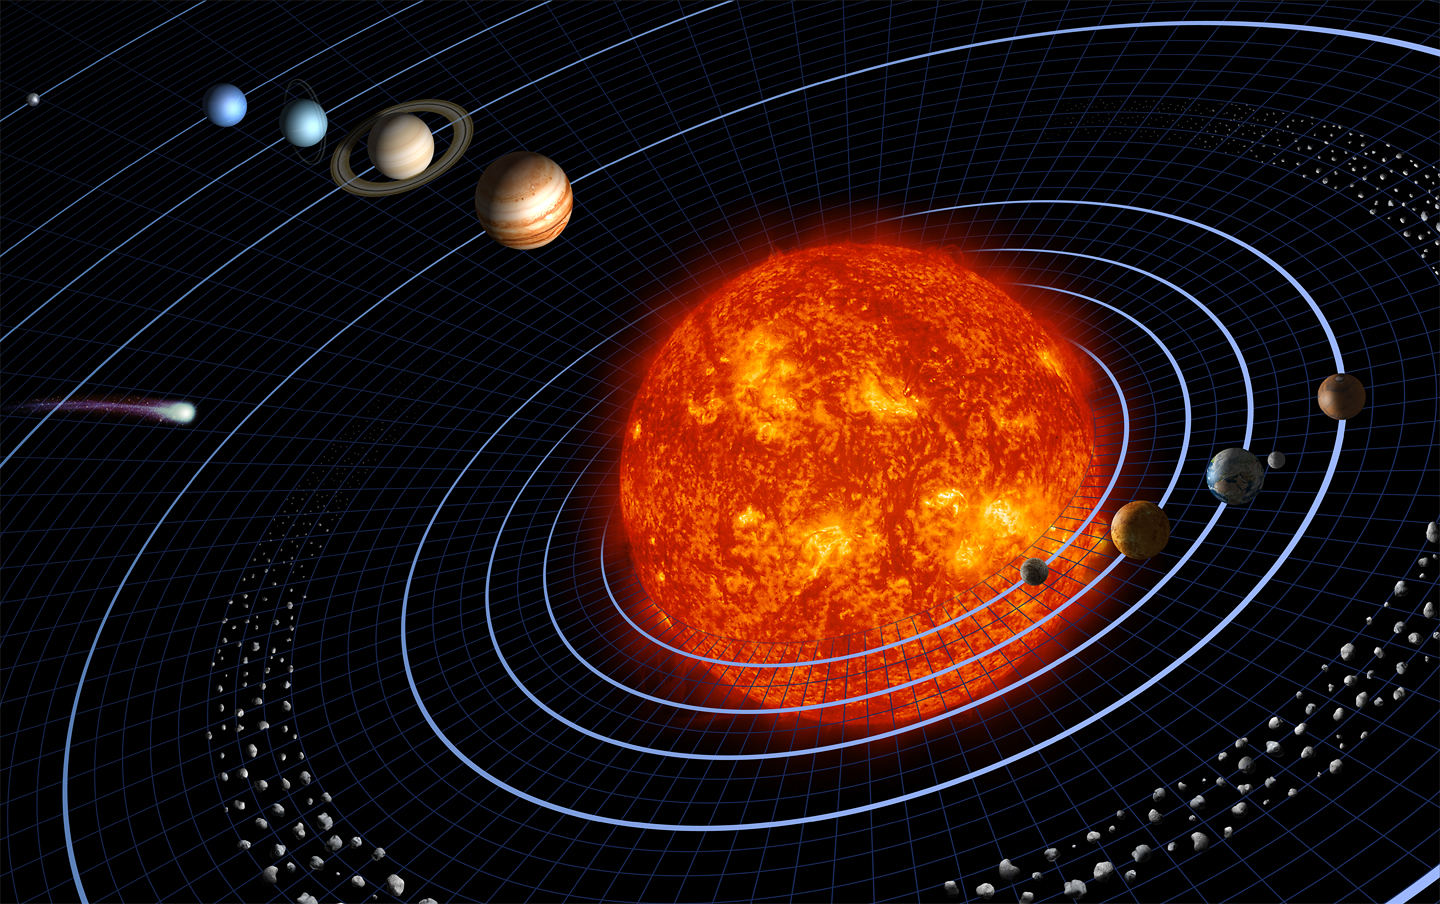
\includegraphics[draft=false,width=0.8\textwidth]{solar_system.jpg}
 \end{center}
\end{minipage}
%\pause
\begin{minipage}{0.48\textwidth}
 \begin{center}
  Reaction and relaxation equations (i.e. blood alcohol content, chemical reaction rates)
 \end{center}
\end{minipage}
%\pause
\vspace{2ex}

\begin{minipage}{0.48\textwidth}
 \begin{center}
  Granular systems

  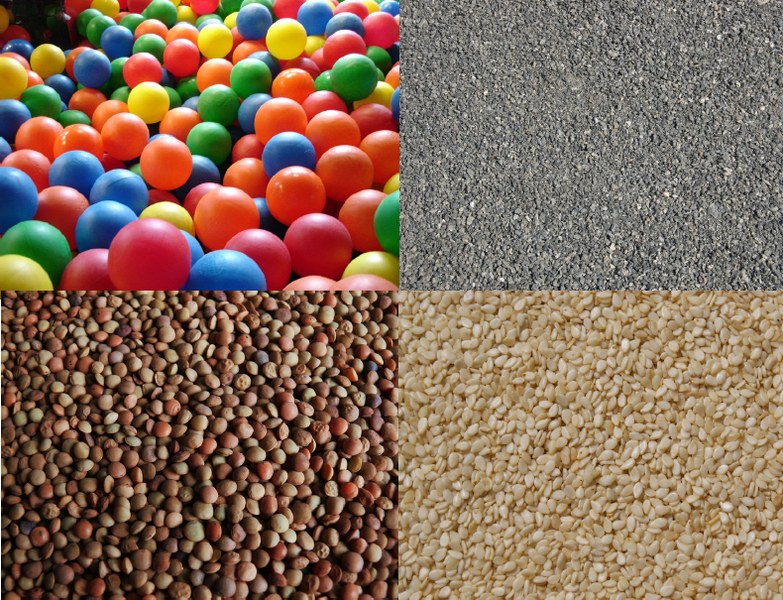
\includegraphics[draft=false,width=0.65\textwidth]{granular_system.png}
 \end{center}
\end{minipage}
%\pause
\begin{minipage}{0.48\textwidth}
 \begin{center}
  Interacting neurons

  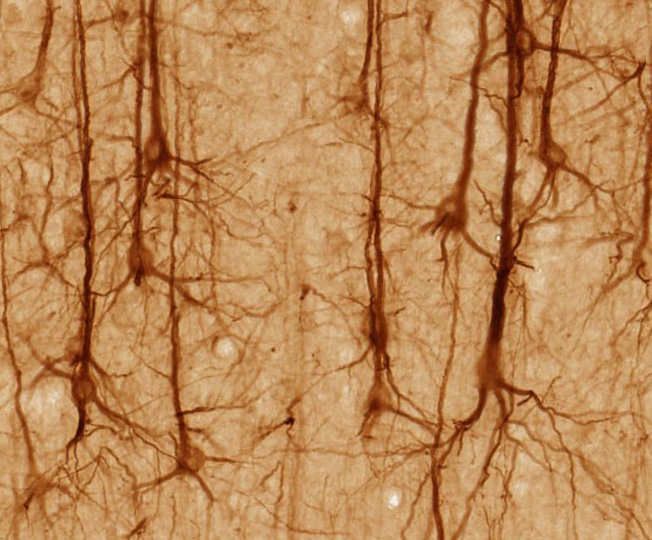
\includegraphics[draft=false,width=0.6\textwidth]{neuron.jpg}
 \end{center}
\end{minipage}
%\pause
\vspace{2ex}

\begin{itemize}
 \item Many examples in physics, biology, chemistry, social sciences
 \item Fundamental in mathematical modelling
\end{itemize}

\end{frame}

\begin{frame}
 
 \heading{What is an ODE?}

 $$\frac{\de x(t)}{\de t} = f\big(x(t) , t\big) \qquad \qquad {\scriptsize \text{short form}} \qquad \dot{x} = f(x,t)
$$

 \begin{itemize}
  \item $x(t)$ -- wanted function (trajectorie)
  \item $t$ -- indenpendent variable (time)
  \item $f(x,t)$ -- defines the ODE, r.h.s
 \end{itemize}

\vspace{4ex}

 Initial Value Problem (IVP):

 $$\dot x = f( x , t ) ,\qquad x(t=0) = x_0$$

\end{frame}


\begin{frame}
  
 \heading{Numerical integration of ODEs}
  
\vspace{4ex}
    Find a numerical solution of an ODE and its IVP
    \[ \dot{x} = f(x,t) \,\,\textrm{,} \quad \quad x(t=0) = x_0\]

   \vspace{2ex}

   Example: Explicit Euler
   \[ x(t + \Delta t ) = x(t) + \Delta t \,\cdot\, f(x(t),t) + \mathcal{O}(\Delta t^2)\]

   \vspace{2ex}

   General scheme of order $s$
    \[ x(t) \,\, \mapsto \,\, x(t+\Delta t) \quad \quad \text{, or}\]
    \[x(t + \Delta t) = \mathcal{F}_t x(t) + \mathcal{O}(\Delta t^{s+1})\]

\end{frame}


\frame{
%  \frametitle{odeint - Solving ODEs in C++}

\heading{\bf \color{red}odeint}

\vspace{2ex}

\centerline{Solving ordinary differential equations in C++}

\vspace{2ex}

Open source
\begin{itemize}
\item Boost license -- do whatever you want do to with it
\item Boost library -- has just been released with v1.53
\end{itemize}

%\pause

\vspace{2ex}

Download
\begin{itemize}
\item \texttt{\textbf{www.odeint.com}}
% \item \texttt{https://github.com/headmyshoulder/odeint-v2}
\end{itemize}

%\pause

\vspace{2ex}

Modern C++
\begin{itemize}
 \item Paradigms: Generic, Template-Meta and Functional Programming
 \item Fast, easy-to-use and extendable.
 \item Container independent
 \item Portable
\end{itemize}

}

\begin{frame}[fragile]
 \heading{Motivation}

 \vspace{2ex}

 We want to solve ODEs $\dot{x}=f(x,t)$ with:
 \begin{itemize}
  \item using  {\tt double}, {\tt std::vector}, {\tt std::array}, \dots as state types.
  \item with complex numbers,
  \item on one, two, three-dimensional lattices, and or on graphs.
  \item on graphic cards.
  \item with arbitrary precision types.
 \end{itemize}

 \vspace{2ex}

Existing libraries support only one state type!

\vspace{4ex}
\centerline{\textbf{Container independent} and {\bf portable} algorithms are needed!}

\end{frame}

\begin{frame}[fragile]

\heading{Example -- Pendulum}

\vspace{2ex}

Pendulum with friction and driving: no analytic solution

\vspace{2ex}

\begin{columns}[T]
  \begin{column}{0.35\textwidth}
    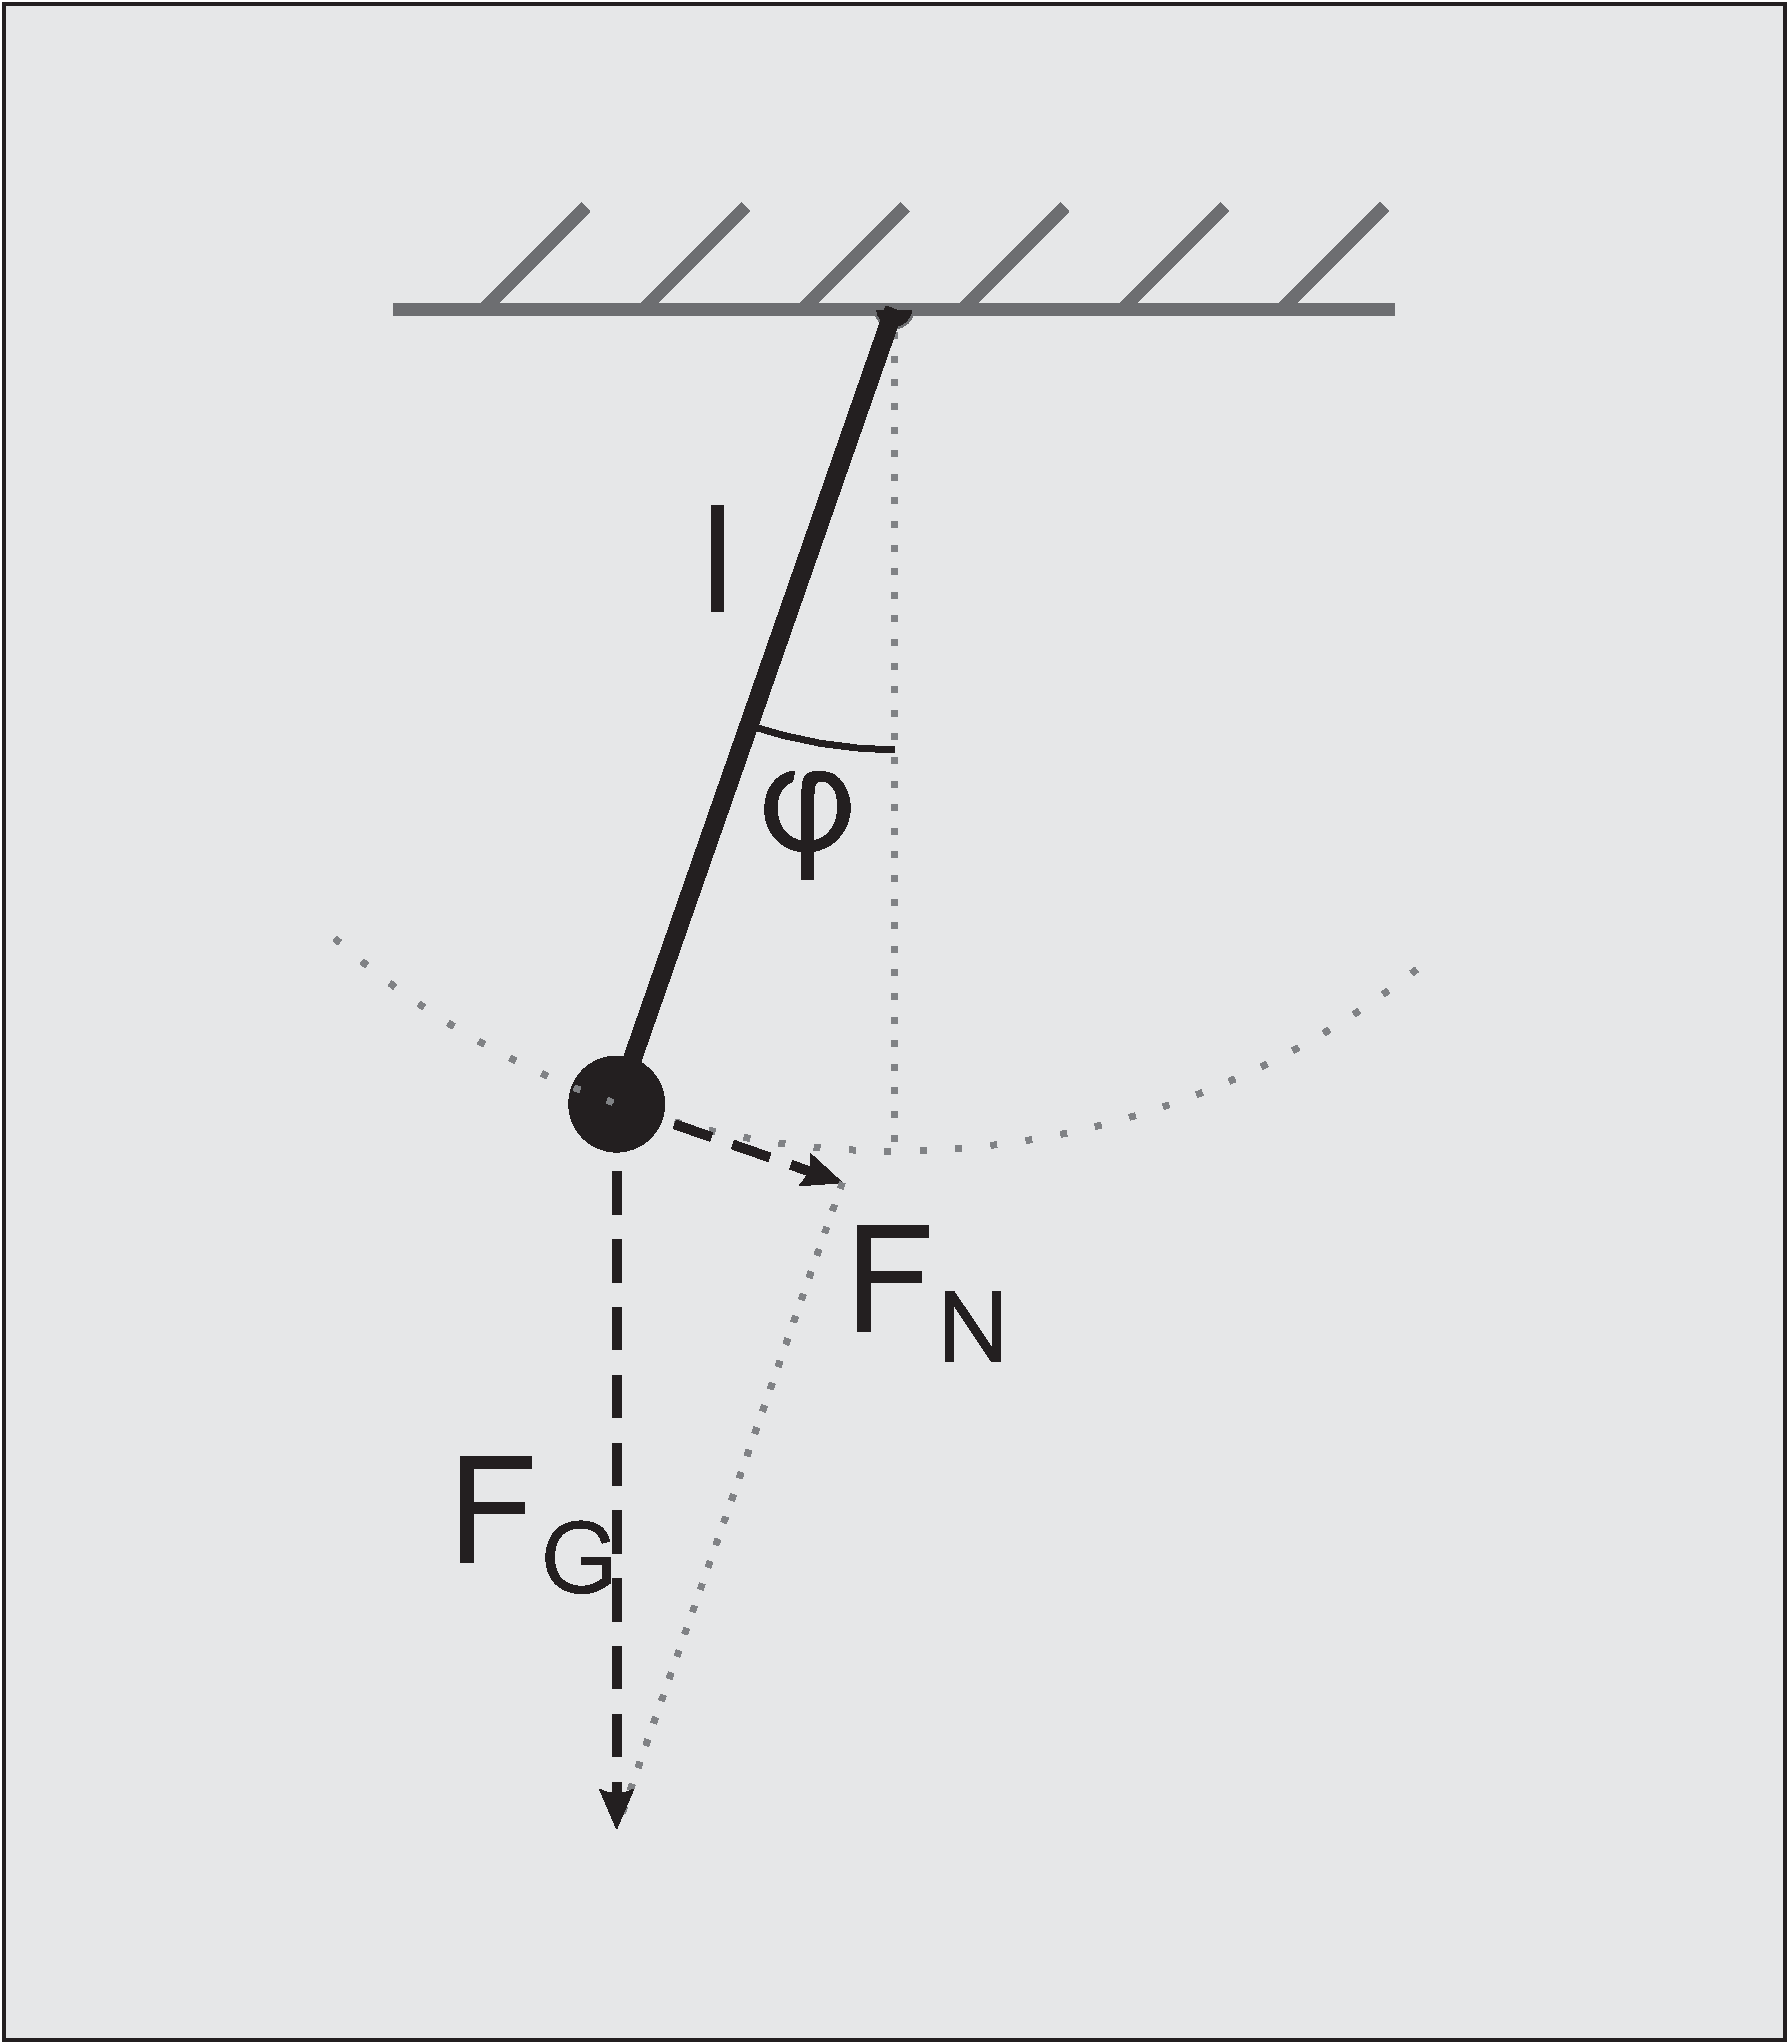
\includegraphics[draft=false,width=1.0\textwidth]{pendulum.pdf}

   \vspace{4ex}
  \end{column}

  \begin{column}{0.65\textwidth}
 $$\ddot{\varphi} = -\omega_0^2 \sin \varphi - \mu \dot{\varphi} + \varepsilon \sin \omega_E t $$

 \vspace{2ex}

 Create a first order ODE

 \vspace{1ex}

 \centerline{$x_1 = \varphi \,\, \text{,} \quad x_2 = \dot{\varphi}$}

 \vspace{-3ex}
 \begin{align*}
   \dot{x_1} &= x_2 \\
   \dot{x_2} &= - \omega_0  \sin x_1 - \mu x_2 + \varepsilon \sin \omega_E t  
 \end{align*}


 $x_1$ and $x_2$ are the state space variables
  
  \end{column}
\end{columns}

 

\end{frame}

\begin{frame}[fragile]

\centerline{ \Large Let's solve the pendulum example numerically}

\vspace{2ex}
\begin{lstlisting}
#include <boost/numeric/odeint.hpp>

namespace odeint = boost::numeric::odeint;
\end{lstlisting}

\vspace{2ex}

\centerline{$\dot{x_1} = x_2 \,\,\text{,} \quad \dot{x_2} = - \omega_0 \sin x_1 - \mu x_2 + \varepsilon \sin \omega_E t$}

\vspace{2ex}
\begin{lstlisting}
typedef std::array<double,2> state_type;
\end{lstlisting}

\end{frame}

\begin{frame}[fragile]

\centerline{ \Large Let's solve the pendulum example numerically}

\vspace{2ex}

$\dot{x_1} = x_2$, $\dot{x_2} = - \omega_0^2 \sin x_1 - \mu x_2 + \varepsilon \sin \omega_E t$ \hspace{6ex} $\omega_0^2 = 1$

\vspace{2ex}

\begin{lstlisting}
struct pendulum
{
  double m_mu, m_omega, m_eps;

  pendulum(double mu,double omega,double eps)
  : m_mu(mu),m_omega(omega),m_eps(eps) { }

  void operator()(const state_type &x,state_type &dxdt,double t) const
  {
    dxdt[0] = x[1];
    dxdt[1] = -sin(x[0]) - m_mu * x[1] +
        m_eps * sin(m_omega*t);
  }
};
\end{lstlisting}

\end{frame}

\begin{frame}[fragile]
 \centerline{ \Large Let's solve the pendulum example numerically}

\vspace{2ex}
$\varphi(0) = x_1(0) = 1 \,\, \text{,} \quad \dot{\varphi}(0) = x_2(0) = 0$
\vspace{2ex}

\begin{lstlisting}
odeint::runge_kutta4< state_type > rk4;
pendulum p( 0.1 , 1.05 , 1.5 );

state_type x = {{ 1.0 , 0.0 }};
double t = 0.0;

const double dt = 0.01;
rk4.do_step( p , x , t , dt );
t += dt;
\end{lstlisting}

\vspace{2ex}

\centerline{$x(0) \mapsto x(\Delta t)$}

\end{frame}

\begin{frame}[fragile]
 \centerline{ \Large Let's solve the pendulum example numerically}

\vspace{1ex}


\begin{lstlisting}
std::cout<<t<<" "<< x[0]<<" "<<x[1]<<"\n";
for( size_t i=0 ; i<10 ; ++i )
{
  rk4.do_step( p , x , t , dt );
  t += dt;
  std::cout<<t<<" "<< x[0]<<" "<<x[1]<<"\n";
}
\end{lstlisting}

\vspace{.5ex}

\centerline{$x(0) \mapsto x(\Delta t) \mapsto x(2\Delta t) \mapsto x(3\Delta t) \mapsto \dots$}

\pause

\vspace{1ex}
\centerline{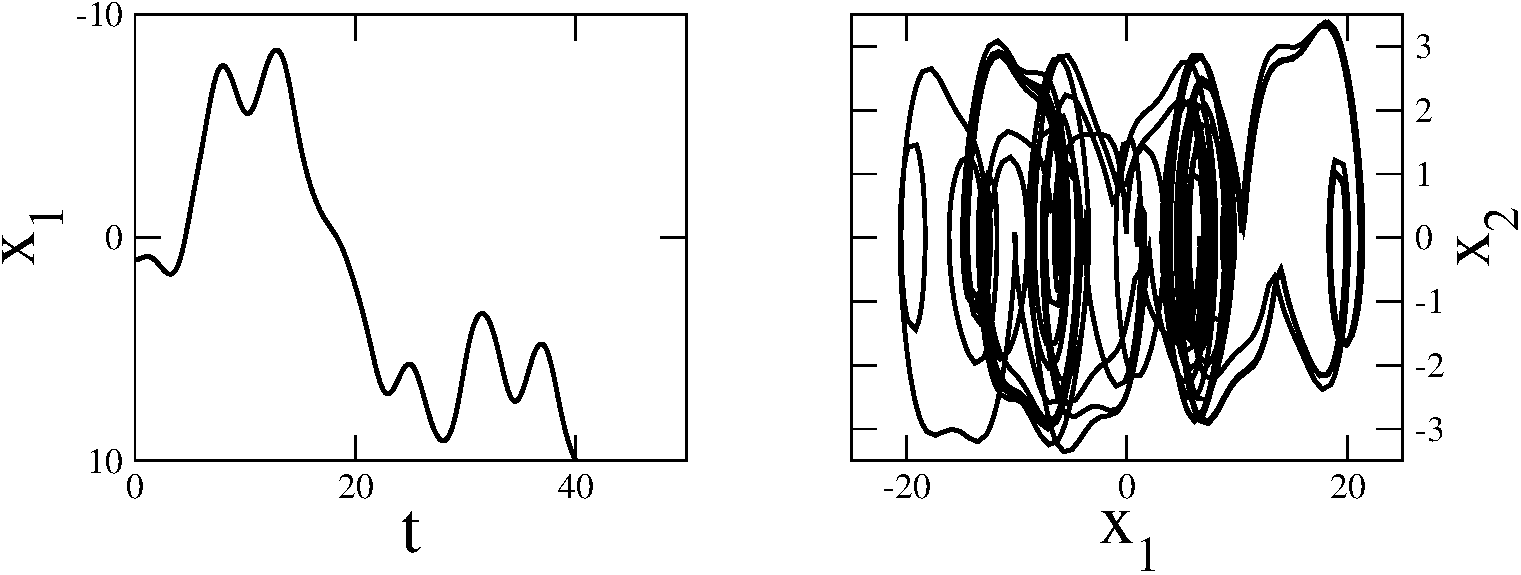
\includegraphics[draft=false,width=0.9\textwidth]{damped_driven.pdf}}

%\centerline{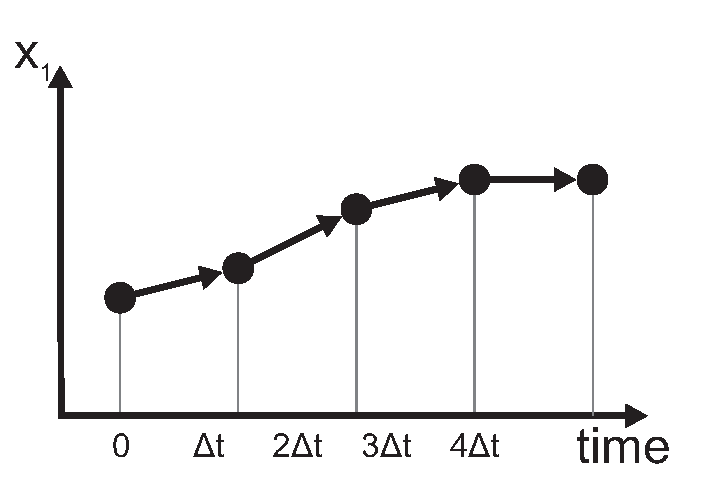
\includegraphics[draft=false,width=0.48\textwidth]{stepper_temporal_evolution.pdf}
%\hspace{1ex}
%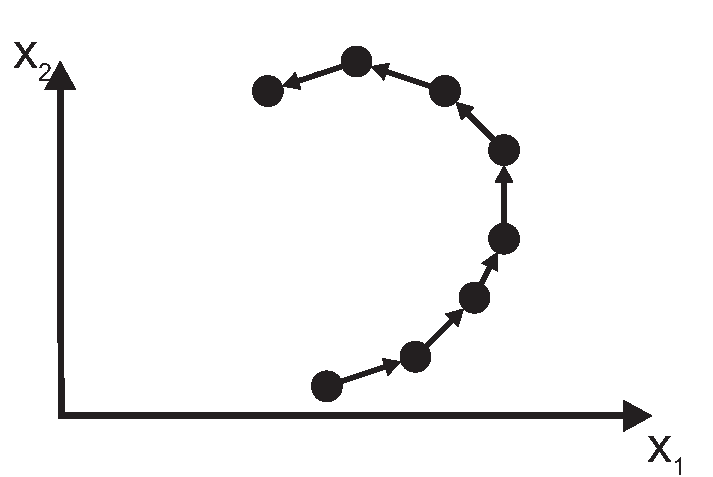
\includegraphics[draft=false,width=0.48\textwidth]{stepper_phase_space.pdf}}
\end{frame}



\begin{frame}
 \heading{Structure of \odeint}
 
 \vspace{2ex}
 \centerline{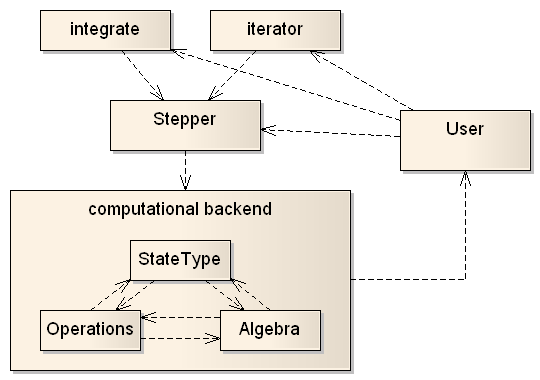
\includegraphics[draft=false,width=0.8\textwidth]{odeint_modularization.png}}

\end{frame}


\begin{frame}
\heading{Independent Algorithms}
\note{To achive maximum flexibility we wanted to implement the numerical algorithms independent from state type and computation details}

\vspace{1em}
\textbf{What?}

Container- and computation-independent implementation of the numerical algorithms.  

\vspace{2em}
\textbf{Why?}

High flexibility and applicability, \odeint\ can be used for virtually any formulation of an ODE.

\vspace{2em}
\textbf{How?}

Detach the algorithm from memory management and computation details and make each part interchangeable.

\end{frame}


\begin{frame}[fragile]
 \heading{Type Declarations}

Tell \odeint\ which types your are working with:

\begin{lstlisting}
/* define your types */
typedef vector<double> state_type;
typedef vector<double> deriv_type;
typedef double value_type;
typedef double time_type;

/* define your stepper algorithm */
typedef runge_kutta4< state_type , value_type , deriv_type , time_type > stepper_type;
\end{lstlisting}

Reasonable standard values for the template parameters allows for:

\begin{lstlisting}
typedef runge_kutta4<state_type> stepper_type;
\end{lstlisting}

\end{frame}


\begin{frame}[fragile]
 \heading{Vector Computations}

\centerline{$\vec x_1 = \vec x_0 + b_1\cdot \Delta t \cdot \vec F_1 + \dots + b_s\cdot \Delta t \cdot \vec F_s$}

\vspace{0.5em}

Split into two parts:

\begin{description}
 \item[1.~Algebra:] responsible for iteration over vector elements
 \item[2.~Operations:] does the mathematical computation on the elements
\end{description}

\vspace{0.5em}

Similar to \lstinline+std::for_each+

\begin{lstlisting}
Algebra algebra;

algebra.for_each3( x1 , x0 , F1 ,
    Operations::scale_sum2( 1.0, b1*dt );
\end{lstlisting}
\pause

The types \lstinline+Algebra+ and \lstinline+Operations+ are template parameters of the steppers, hence exchangeable.
\end{frame}

\begin{frame}[fragile]

%\lstinline+range_algebra & default_operations+ can be used with any Container that supports Boost.Range and whose \lstinline+container::value_type+ supports operators \lstinline!+,*!.

For example \lstinline+vector< double >+:
\begin{lstlisting}
typedef vector< double > state_type;
typedef vector< double > deriv_type;
typedef double value_type;
typedef double time_type;

typedef runge_kutta4< state_type , value_type , 
                      deriv_type , time_type , 
                      range_algebra , 
                      default_operations 
                    > stepper_type
\end{lstlisting}

\vspace{1em}
As these are also the default values, this can be shortened:
\begin{lstlisting}
typedef runge_kutta4<state_type> stepper_type; 
\end{lstlisting}

\end{frame}

\begin{frame}[fragile]
 \heading{Other Algebras}

 \vspace{1ex}
 
 Additional computation backends included in odeint:
 
\begin{description}
 \item[array\_algebra:] for \lstinline+std::array+, faster than range\_algebra for some compilers.
 \item[vector\_space\_algebra:] for \lstinline+state_types+ that have operators \lstinline!+,*! defined.
 \item[fusion\_algebra:] works with compile-time sequences like \lstinline+fusion::vector+ of Boost.Units
 \item[thrust\_algebra \& thrust\_operations:] Use thrust library to perform computation on CUDA graphic cards
 \item[mkl\_operations:] Use Intel's Math Kernel Library
 %\item[nested\_algebra:] can handle nested containers that support Boost.Range, e.g.\ \lstinline+vector< vector<double> >+
\end{description}

See tutorial and documentation on \verb+www.odeint.com+ for more.

\end{frame}


\begin{frame}[fragile]
 \heading{Conclusion}

\vspace{2ex}

odeint is a modern C++ library for solving ODEs that is
%odeint is a modern C++ library for solving ordinary differential equations, which is

\begin{itemize}
 \item easy-to-use
 \item highly-flexible
 \begin{itemize}
  \item data types (topology of the ODE, complex numbers, precision, \dots)
  \item computations (CPU, CUDA, OpenMP, ...)
 \end{itemize}
 \item fast
\end{itemize}


\vspace{1ex}

Used by:
\vspace{1ex}

\textbf{NetEvo} -- Simulation dynamical networks\\
\textbf{OMPL} -- Open Motion Planning Library\\
\textbf{icicle} -- cloud/precipitation model\\
\textbf{Score} -- Smooth Particle Hydrodynamics Simulation (com.)\\
\textbf{VLE} -- Virtual Environment Laboratory (planned to use \odeint )\\

\vspace{1ex}
Several research groups

\end{frame}


\begin{frame}
 \heading{Roadmap}

 \vspace{2ex}

Near future:
\begin{itemize}
\item Implicit steppers
\item Multiprozessor backends (OpenMP, MPI, HPX)
\end{itemize}

\vspace{2ex}
Further plans:
\begin{itemize}
 \item Dormand-Prince 853 steppers
 \item More algebras: cublas, TBB, Boost SIMD library
\end{itemize}

\vspace{2ex}                                                                                                       
Perspective:
\begin{itemize}
 \item C++11 version
 \item sdeint -- methods for stochastic differential equations
 \item ddeint -- methods for delay differential equations
\end{itemize}


\end{frame}

\end{document}